\chapter{\label{ch:pdj}Personagem do Jogador}

O RPG de Mesa terá dois tipos de personagens: 
\begin{itemize}
	\item Personagens do Mestre (PdM's ou NPC): Os PdM's são criados e controlados pelo narrador da mesa. A criação de PdM's é apresentada no Capítulo~\ref{ch:mestre} - \emph{Área do Mestre}.

	\item Personagem do Jogador (PdJ): O PdJ é criado e controlado por um dos jogadores da mesa. Cada jogador controla pelo menos um personagem.
\end{itemize}

\section{\label{sec:pdj}Criando um PdJ}

Para criar um PdJ no Sistema +2d6@ifsul, recomenda-se fazer primeiro uma descrição em texto de como é este personagem. Todas estas características serão transformadas em valores numéricos registrados na Ficha de Personagem. Logicamente, quanto maior o valor numérico nestes elementos, mais poderoso é o personagem naquele aspecto.

Os principais pontos da ficha são: 

\begin{itemize}
	\item ATRIBUTOS: Explicados na seção~\ref{subsecAtributos}, representam as capacidades físicas e mentais do personagem.
	\item PERÍCIAS: Explicadas na seção~\ref{subsecPericias}, são habilidades/ofícios aprendidas/conquistadas pelo personagem antes da aventura. Novas perícias também poderão ser aprendidas durante a aventura, principalmente quando estas forem longas no formato de campanhas.
	\item VANTAGENS e DESVANTAGENS: Explicadas na seção~\ref{subsecVantagens}, são características/poderes que afetam o personagem. Vantagens auxiliam/ajudam em determinadas situações, enquanto desvantagens prejudicam/atrapalham.
\end{itemize}

A Figura~\ref{fichaMaoLivre} mostra uma Ficha de Personagem feita a mão livre. O Apêndice~\ref{apendiceFichas} mostra dois outros modelos para Ficha de personagem. 

\begin{figure}[htb]
	\centering
	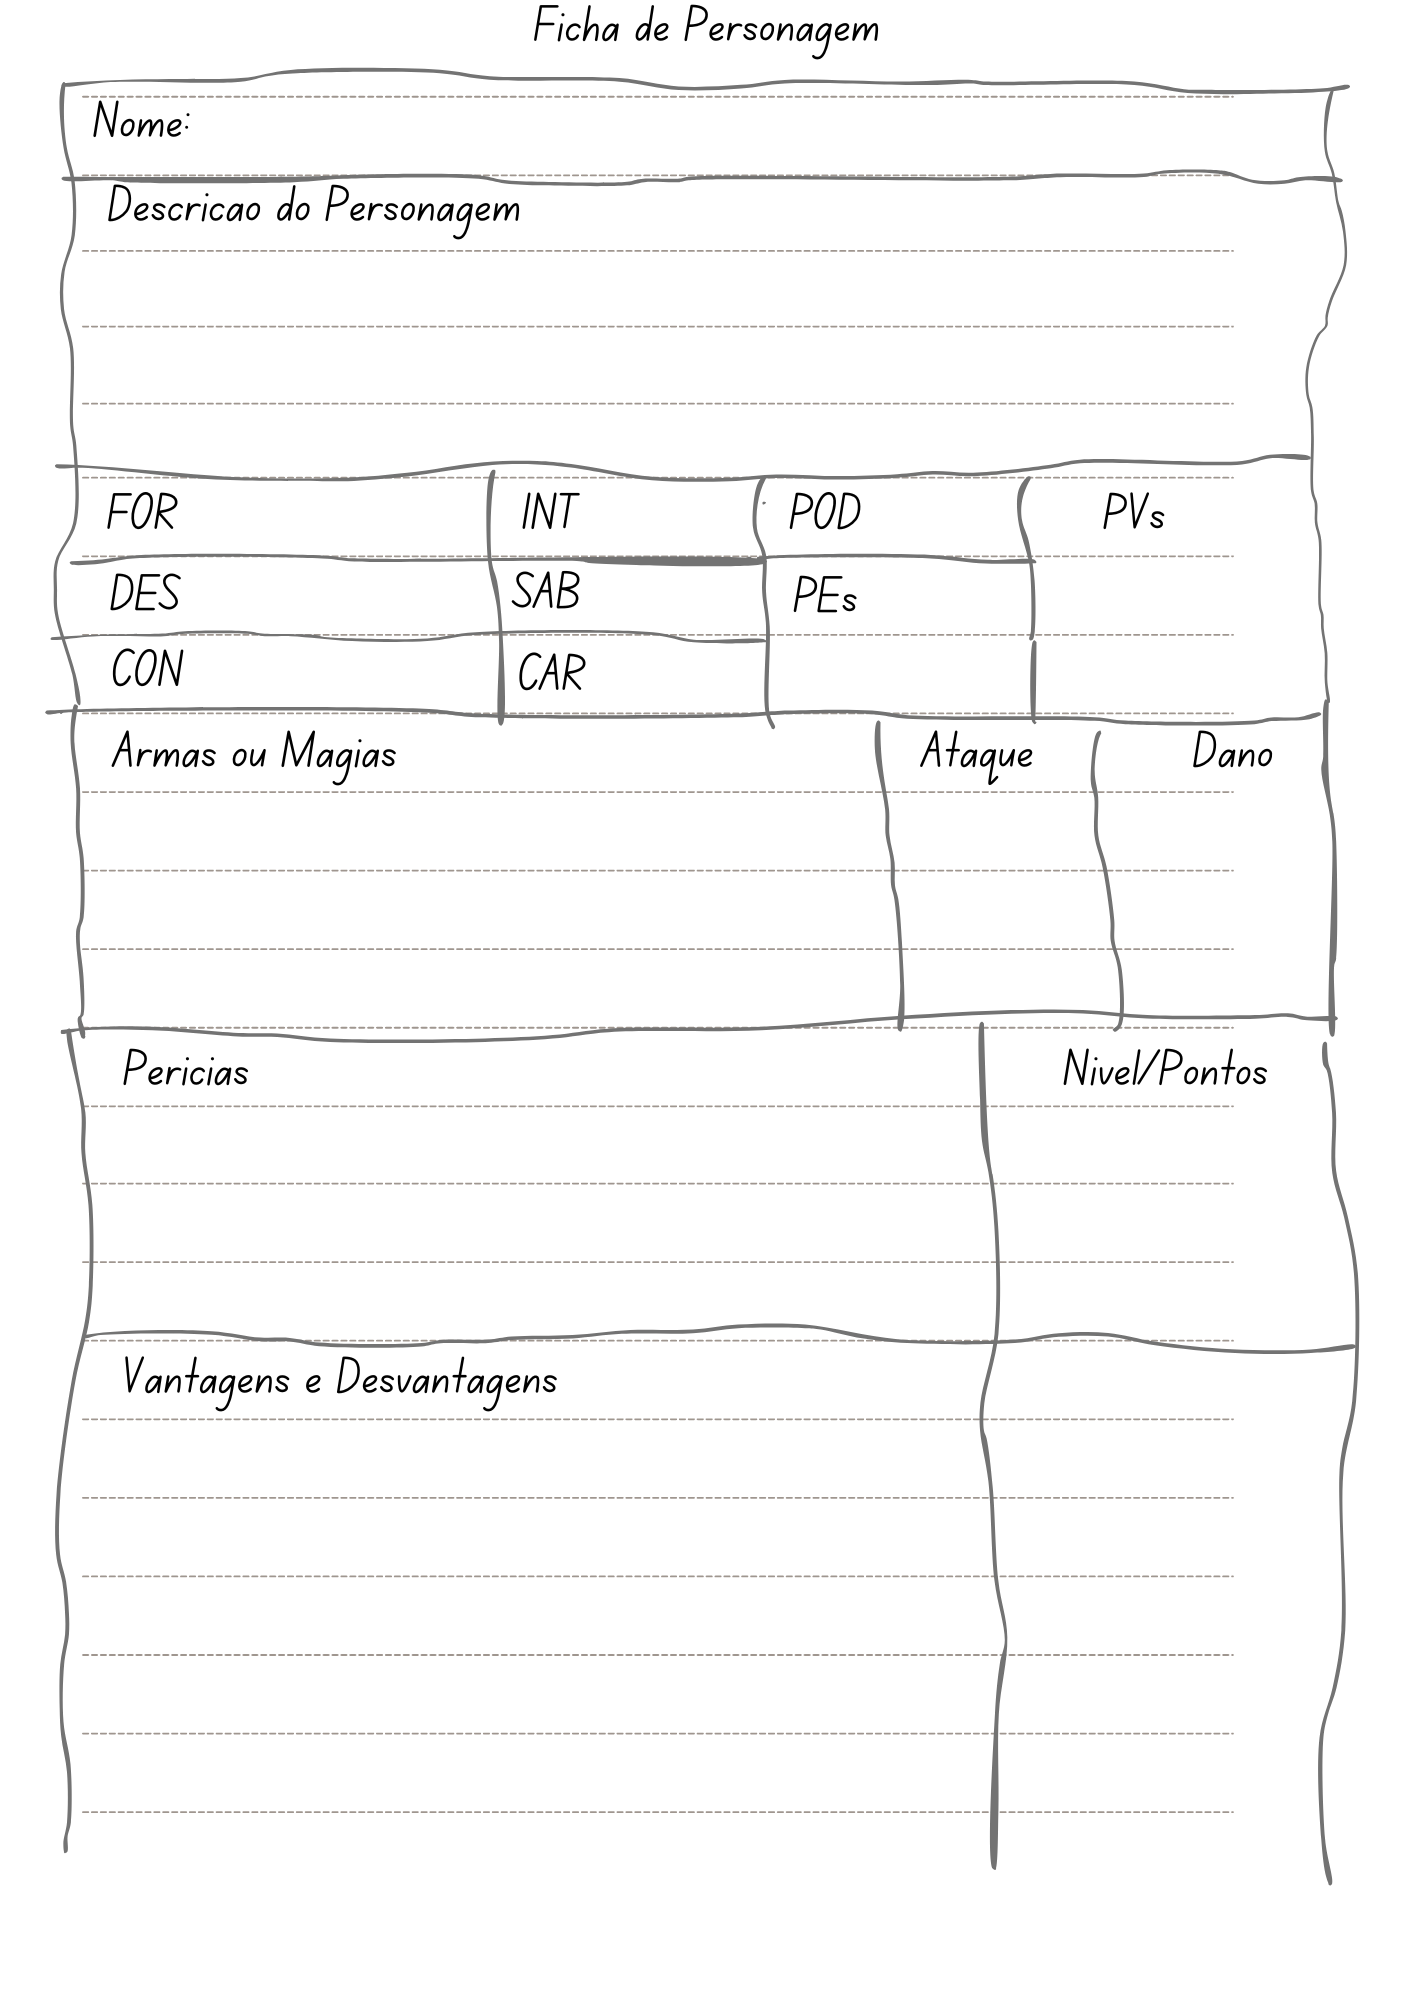
\includegraphics[scale=0.5]{img/fichaManual.png}
	\caption{Exemplo de ficha feita a mão livre.}
	\label{fichaMaoLivre}
\end{figure}

\subsection{\label{subsecAtributos}Atributos}

\subsection{\label{subsecPericias}Perícias}
\subsection{\label{subsecVantagens}Vantagens e Desvantagens}